\section{LLM-aided KG Construction}
In this section, we study and establish the advantages of utilizing LLMs for the construction of KGs, by demonstrating their effectiveness in improving the \textit{accuracy}, \textit{consistency}, \textit{coverage}, and \textit{freshness} of knowledge. %Generally speaking, current research and practice on KGs are intensive but mostly around specific types of entities. 
Popular KGs such as Freebase \cite{bollacker2008freebase}, Yago \cite{suchanek2008yago} and Wikidata \cite{vrandevcic2014wikidata} contain hundreds of millions of real-world entities like people, places, and things, along with their multi-typed relations. However, since the KGs are collected and curated by different platforms and institutions, they do not use a unified coding system or thesaurus. The varying terminologies due to different conventions or abbreviations can lead to high degrees of duplication and inconsistency when multiple KGs are directly put together. 
Moreover, the sheer amounts of data in existing KGs are enormous, but the knowledge is still never comprehensive enough to serve various needs of real-world applications, especially those requiring rapidly updated knowledge.
%A few studies have attempted to construct general-purpose healthcare KGs through integrating existing ones \cite{su2023biomedical, cornet2008forty, santos2020clinical}, but they heavily rely on existing coding systems and thesauruses \cite{harrison2021icd, lipscomb2000medical, bodenreider2004unified} for entity alignment across KGs, which often fail in front of varying terminologies such as due to different conventions or abbreviations, leading to high degrees of duplication and inconsistency. 
Recently, pioneering studies including ours have demonstrated strong promise of utilizing LLMs to automate the construction, integration, and enrichment of KGs \cite{zhu2023llms, ye2022generative, qin2023chatgpt, kommineni2024human, zhang2024extract, vizcarra2024representing, yu2023bear, hu2023llm, meyer2023llm, hofer2024towards, yang2024graphusion}. In the following, we give several examples of promising attempts of these kinds and discuss more natural use cases of LLMs and multi-modal foundation models (MMFMs) toward constructing high-quality KGs as promising future directions. 

\subsection{Integrating existing KGs}
% \carl{Need some overviews about motivation, challenge, why LLMs are promising, recent works using LLMs (ours), other recent works, future directions}
%HiPrompt, PromptLink and other LLM-based KG integration
KG integration, also known as knowledge fusion or knowledge alignment, represents a fundamental challenge in the broader landscape of knowledge engineering, which involves integrating multiple KGs that originate from varied sources and formats~\cite{yan2024knownet,lu2022open}.
% The integration of existing KGs presents both great premise and significant challenges in knowledge engineering. 
While individual KGs often excel in specific domains or use cases, their true potential can be unlocked through effective integration, enabling more comprehensive and robust knowledge representation~\cite{himmelstein2017systematic,santos2020clinical}. 
As the number and diversity of KGs continue to grow, the need for effective integration methods becomes increasingly critical.

However, the integration of existing KGs faces several key challenges: (1) \textit{semantic heterogeneity across sources}: Different KGs often use varying terminologies, definitions, and contextual frameworks to represent similar concepts~\cite{liu2022selfkg}; 
(2) \textit{varying granularity levels in knowledge representation}: KGs may differ in the detail and depth with which they describe entities and relationships, impacting the consistency and usability of integrated data. 
Although several neural approaches have been proposed for entity alignment on KGs~\cite{wang2018cross,zhu2020collective,yan2021dynamic}, these methods generally depend heavily on labeled data for training. However, obtaining sufficient labeled data often involves substantial manual effort and can be rather costly.

LLMs have emerged as a promising solution to these challenges with unique advantages: 
First, their strong natural language understanding capabilities enable them to capture semantic relationships among concepts that may be missed by traditional string-matching or embedding-based approaches \cite{chen2023dipping}. 
Second, LLMs can draw on their extensive knowledge acquired during pre-training to aid in disambiguating entities and mapping relationships across different KGs \cite{sancheti2024llm}.
Third, LLMs possess robust few-shot learning abilities, making them particularly valuable for specialized domain applications where labeled data are limited \cite{brown2020language,agrawal2022large}.

\begin{figure}[htbp]
    \begin{center}
    %\framebox[4.0in]{$\;$}
    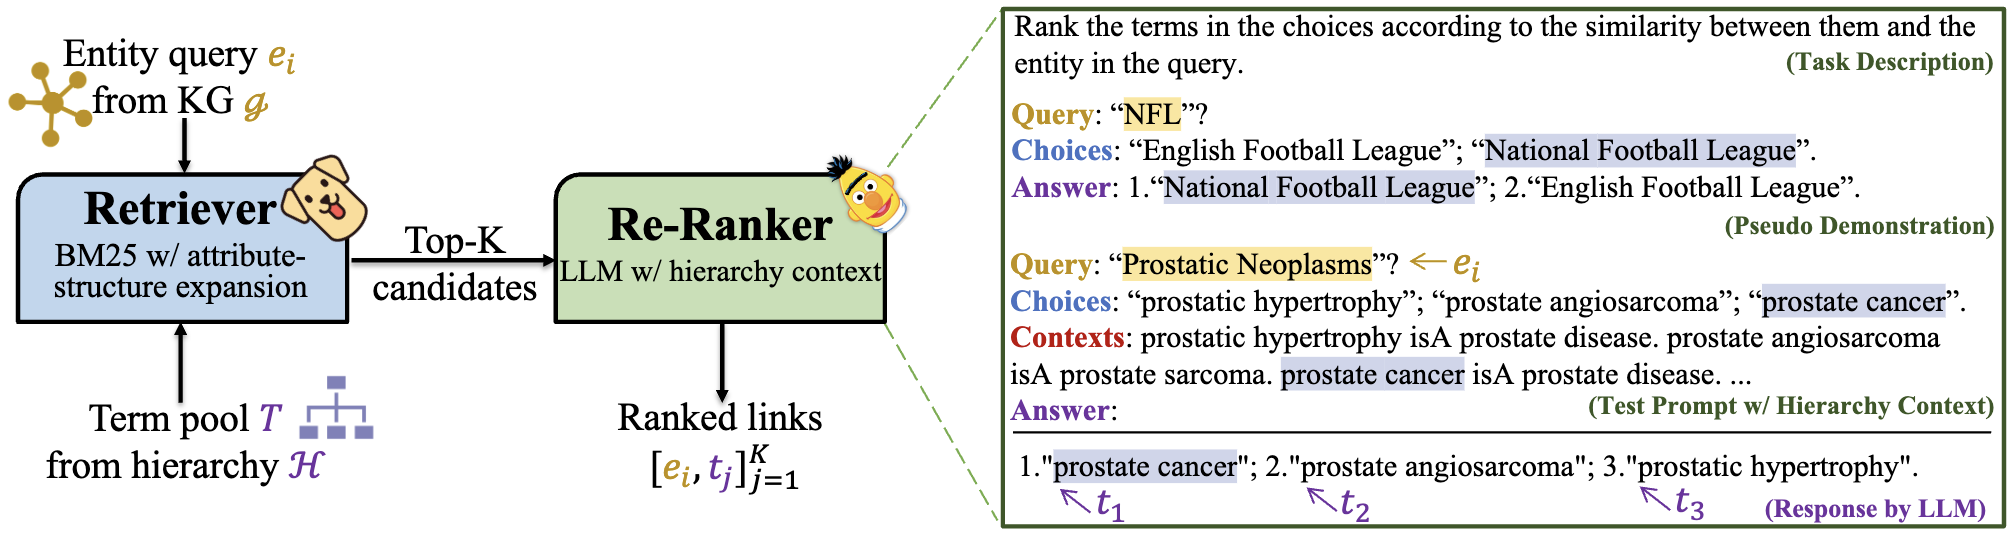
\includegraphics[width=.95\columnwidth]{submissions/CarlYang2024/figures/hiprompt.png}
    \end{center}
    \vspace{-4mm}
    \caption{The overall framework of Hiprompt.}
    \label{fig:hiprompt}
     \vspace{-2mm}
\end{figure}

Recent work has demonstrated the effectiveness of LLM-based approaches in KG integration. 
For example, Lu et al.~\citep{lu2023hiprompt} developed HiPrompt (framework shown in Figure~\ref{fig:hiprompt}), which aligns entities between biomedical KGs and standardized hierarchical entity taxonomies. 
This task poses significant challenges due to the scarcity of available pairs and the inconsistent naming conventions between KGs and entity taxonomies.
Their two-stage approach combines traditional information retrieval techniques (BM25) with LLM-based re-ranking using hierarchy-oriented prompts, achieving superior performance in few-shot biomedical knowledge-graph integration.  
Building on this direction, Xie et al.~\citep{xie2024promptlink} developed PromptLink, a framework that leverages both domain-specific language models and GPT-4 for cross-source biomedical concept linking. The framework employs a two-stage prompting mechanism by first eliciting the biomedical prior knowledge from the LLM for the concept linking task and then enforcing the LLM to reflect on its own predictions to further enhance their reliability. 
PromptLink’s success in zero-shot scenarios illustrates the potential of LLMs to generalize across diverse data sources without extensive training data.

In contrast to the two LLM approaches that primarily use LLMs for ranking candidate sets, AutoAlign \cite{zhang2023autoalign} employs off-the-shelf LLMs to construct a predicate-proximity graph that captures relationships between entity types rather than individual entities. It then aligns the entity embeddings of two KGs into a common vector space by calculating similarity based on entity attributes.


These advances suggest several promising future directions for LLM-aided KG integration. For example, LLMs could potentially facilitate the continuous integration of new knowledge into existing KGs dynamically and automatically by identifying and resolving conflicts between new and existing information, while maintaining consistency across the integrated knowledge base. Such real-time data integration is especially beneficial for dynamic applications like live event monitoring and real-world decision-making. {Furthermore, integrating KGs with LLMs remains challenging due to the risk of generating false or untrustworthy information~\cite{yang2024give}. To mitigate this issue, there is a growing need for improved human-in-the-loop systems. Specifically, enhanced interfaces~\cite{hassan2017claimbuster,nakov2021automated} can enable experts to more effectively verify and interpret LLM-generated recommendations, ensuring greater reliability and transparency.}



% Lu et al.~\citep{lu2023hiprompt} propose HiPrompt, an innovative framework that leverages LLMs for biomedical knowledge fusion. Their work addresses the challenge of aligning entities from biomedical KGs with terms in a standardized hierarchical index system, a task that traditionally suffers from scarce labeled data and inconsistent naming conventions. HiPrompt employs a two-stage approach: a retrieval module using BM25 with expanded entity and term representations, followed by an LLM-based re-ranking module that utilizes hierarchy-oriented prompts. This approach enables effective few-shot learning, outperforming both conventional unsupervised methods and neural embedding models in zero-shot and one-shot settings. It demonstrates the potential of LLMs in capturing complex semantic relationships and hierarchical constraints in KG integration tasks, even with minimal supervision. Their findings suggest that LLM-aided approaches could significantly advance the field of KG construction and integration, particularly in domains with limited labeled data.

% Another notable example is PromptLink~\citep{xie2024promptlink}, which leverages LLMs for cross-source biomedical concept linking. PromptLink combines the strengths of biomedical-specialized pre-trained language models and GPT-4 to address the challenges of inconsistent naming conventions across different data sources. The framework employs a two-stage prompting mechanism that efficiently filters candidates and generates reliable linking predictions, including NIL predictions when no suitable match is found. By outperforming conventional string-matching and machine learning-based methods in zero-shot accuracy, PromptLink demonstrates the potential of LLMs in enhancing KG integration tasks. This approach is particularly valuable in domains where labeled data is scarce and the ability to generalize across various data sources is crucial.

\subsection{Constructing and Completing KGs}
KGs have high-standard requirements on the quality of knowledge, regarding accuracy, consistency, coverage and freshness. No matter constructed through manual curation, NLP tools, or their combinations, KGs can unavoidably include erroneous knowledge. Moreover, when multiple KGs are integrated, conflicting knowledge can emerge. Finally, new knowledge is constantly generated from new experiments and research, making existing knowledge inaccurate and incomplete. LLMs have emerged as a promising solution, leveraging the vast and adaptable knowledge acquired during pre-training to overcome these limitations \cite{petroni2019language, yu2024kola, xu2024clingen, alkhamissi2022review}. 
The key advantage of LLMs for KG construction and completion is their ability to generate novel, semantically coherent information with minimal reliance on additional labeled data.

% The key advantage of LLMs in this domain lies in their ability to generate novel, semantically coherent information that can supplement and enrich existing KGs. Unlike rule-based or supervised machine learning approaches, LLMs can leverage their extensive understanding of language and the world to infer missing connections, identify new entities, and uncover implicit relationships - all without being constrained by the limitations of manually curated training data.

Recent studies have highlighted the effectiveness of LLM-based approaches for KG construction and completion. Zhu et al. \citep{zhu2023llms} utilize in-context learning capabilities of LLMs to complete tuples with missing entities or relations to generate new knowledge triplets for augmenting existing KGs.
Wei et al. \citep{wei-etal-2023-kicgpt} and Wang et al. \citep{wang-etal-2024-kc} tackle KG completion as a candidate identification and ranking task, proposing a “retrieve-rank” pipeline where LLMs are used to rerank top-retrieved entities, thus creating additional knowledge triplets.

An alternative approach to prompting LLMs involves using code-based prompts,  rather than natural language, to incorporate new entities into existing KGs~\cite{bi2024codekgc,zeng2024codetaxo}. 
Code LLMs, extensively trained on structured data such as programming code, are inherently well-suited to the structured nature of KGs.
Using a code-based interface enables more effective handling of graph-like structures, logical relationships, and precise reasoning~\cite{madaan2022language,chen2023program,shi2024agent}.
Specifically, Bi et al. \cite{bi2024codekgc} first encoded the schema of KGs by modeling code definitions, to capture the structural information inherent in the data. They then employed chain-of-thought prompting to produce accurate knowledge triples. This methodology demonstrates improved performance over traditional natural language-based prompts. 
Similarly, Zeng et al.~\citep{zeng2024codetaxo} proposed CodeTaxo, which represents entities within a base 'Entity' class, mirroring hierarchical relationships in programming constructs. This approach enables LLMs to efficiently create taxonomic structures by leveraging syntactic capabilities commonly used in code tasks, thus enhancing the organization and completeness of KGs. 
% Another notable example is CodeTaxo~\citep{zeng2024codetaxo} which encapsulates entities in a base class 'Entity' to better characterize hierarchical relations similar to programming constructs. This enables the LLM to efficiently process and generate taxonomic structures by leveraging its strong syntactic capabilities, which are typically associated with code understanding tasks. By combining the LLM's natural language understanding with its code-related skills, CodeTaxo demonstrates the versatility of these models in enhancing the completeness and organization of KGs.


The above methods primarily focus on prompting LLMs for KG construction and completion. While these methods show promise, they fall short in fully adapting LLMs to target tasks and can suffer from hallucination issues. To address these limitations, several studies aim to improve the quality of LLM-generated content for KG tasks. 
{Zhang et al. \cite{zhang2024extract} presented a three-phase framework for constructing KGs with LLMs to enhance contextual understanding and schema alignment. 
It starts with open information extraction to identify relation triplets from unlabeled textual corpora, followed by schema definition where LLMs generate contextually relevant descriptions for schema components. 
Finally, the extracted triplets are aligned with the schema.  
To further enhance the quality of the extracted
triplets and minimize the risk of misinformation, a schema retriever is used to generate a list of candidate entities and relations to guide the triplet extraction steps. This approach works for both predefined schemas and situations where the schema needs to be inferred from the context.
}
% \cite{zhang2024extract} presents a three-phase framework for constructing KGs with LLMs to enhance contextual understanding and schema alignment. The process begins with open information extraction, where relational triplets are identified from unlabeled textual corpora. Next, LLMs is used to define schema components by generating contextually relevant, human-like descriptions. In the final canonicalization phase, extracted triplets are aligned with the schema to ensure consistency and reduce redundancy. This adaptable framework is effective in both predefined schema settings and scenarios where schema must be inferred from context.
Additionally, various studies explored fine-tuning LLMs specifically for KG completion. Zhang et al.~\cite{kopa} proposed KOPA that first applies structural pre-training to create embeddings of entities and relations in KGs, and project embeddings into the textual space as virtual knowledge tokens. These tokens act as prefixes in LLM input prompts, enabling structure-aware reasoning that leverages both the generative power of LLMs and the retrieval of structured KG information to improve the accuracy and completeness of KG completion tasks. 
Jiang et al.~\citep{jiang2024kg} introduced KG-FIT for using open-world knowledge from LLMs to enhance KG embeddings. It initially constructs a semantically coherent, hierarchical structure of entity clusters, guided by LLM-powered entity representations. It then fine-tunes these embeddings by integrating the hierarchical structure with textual embeddings. This hybrid approach allows KG-FIT to capture both the semantic depth of LLMs and the structural information intrinsic to KGs, resulting in more comprehensive KG representations.



% TaxoPrompt~\citep{xu2022taxoprompt}, a prompt-based method for self-supervised taxonomy expansion that effectively leverages the global structure of taxonomies. TaxoPrompt integrates the taxonomic context into the training of a language model (LM) by employing a customized random walk algorithm that captures relational paths within the taxonomy. This context is then used in a prompt-tuning framework to transform the taxonomy expansion problem into a hypernym generation task. During the process, a template creates a cloze task where the LM predicts missing hypernyms based on provided context, thus maintaining the structural integrity of the taxonomy.


% https://arxiv.org/abs/2405.16412
% https://dl.acm.org/doi/pdf/10.1145/3637528.3671469
% https://arxiv.org/pdf/2408.09070
% https://www.ijcai.org/proceedings/2022/0615.pdf

\begin{figure}[htbp]
    \begin{center}
    %\framebox[4.0in]{$\;$}
    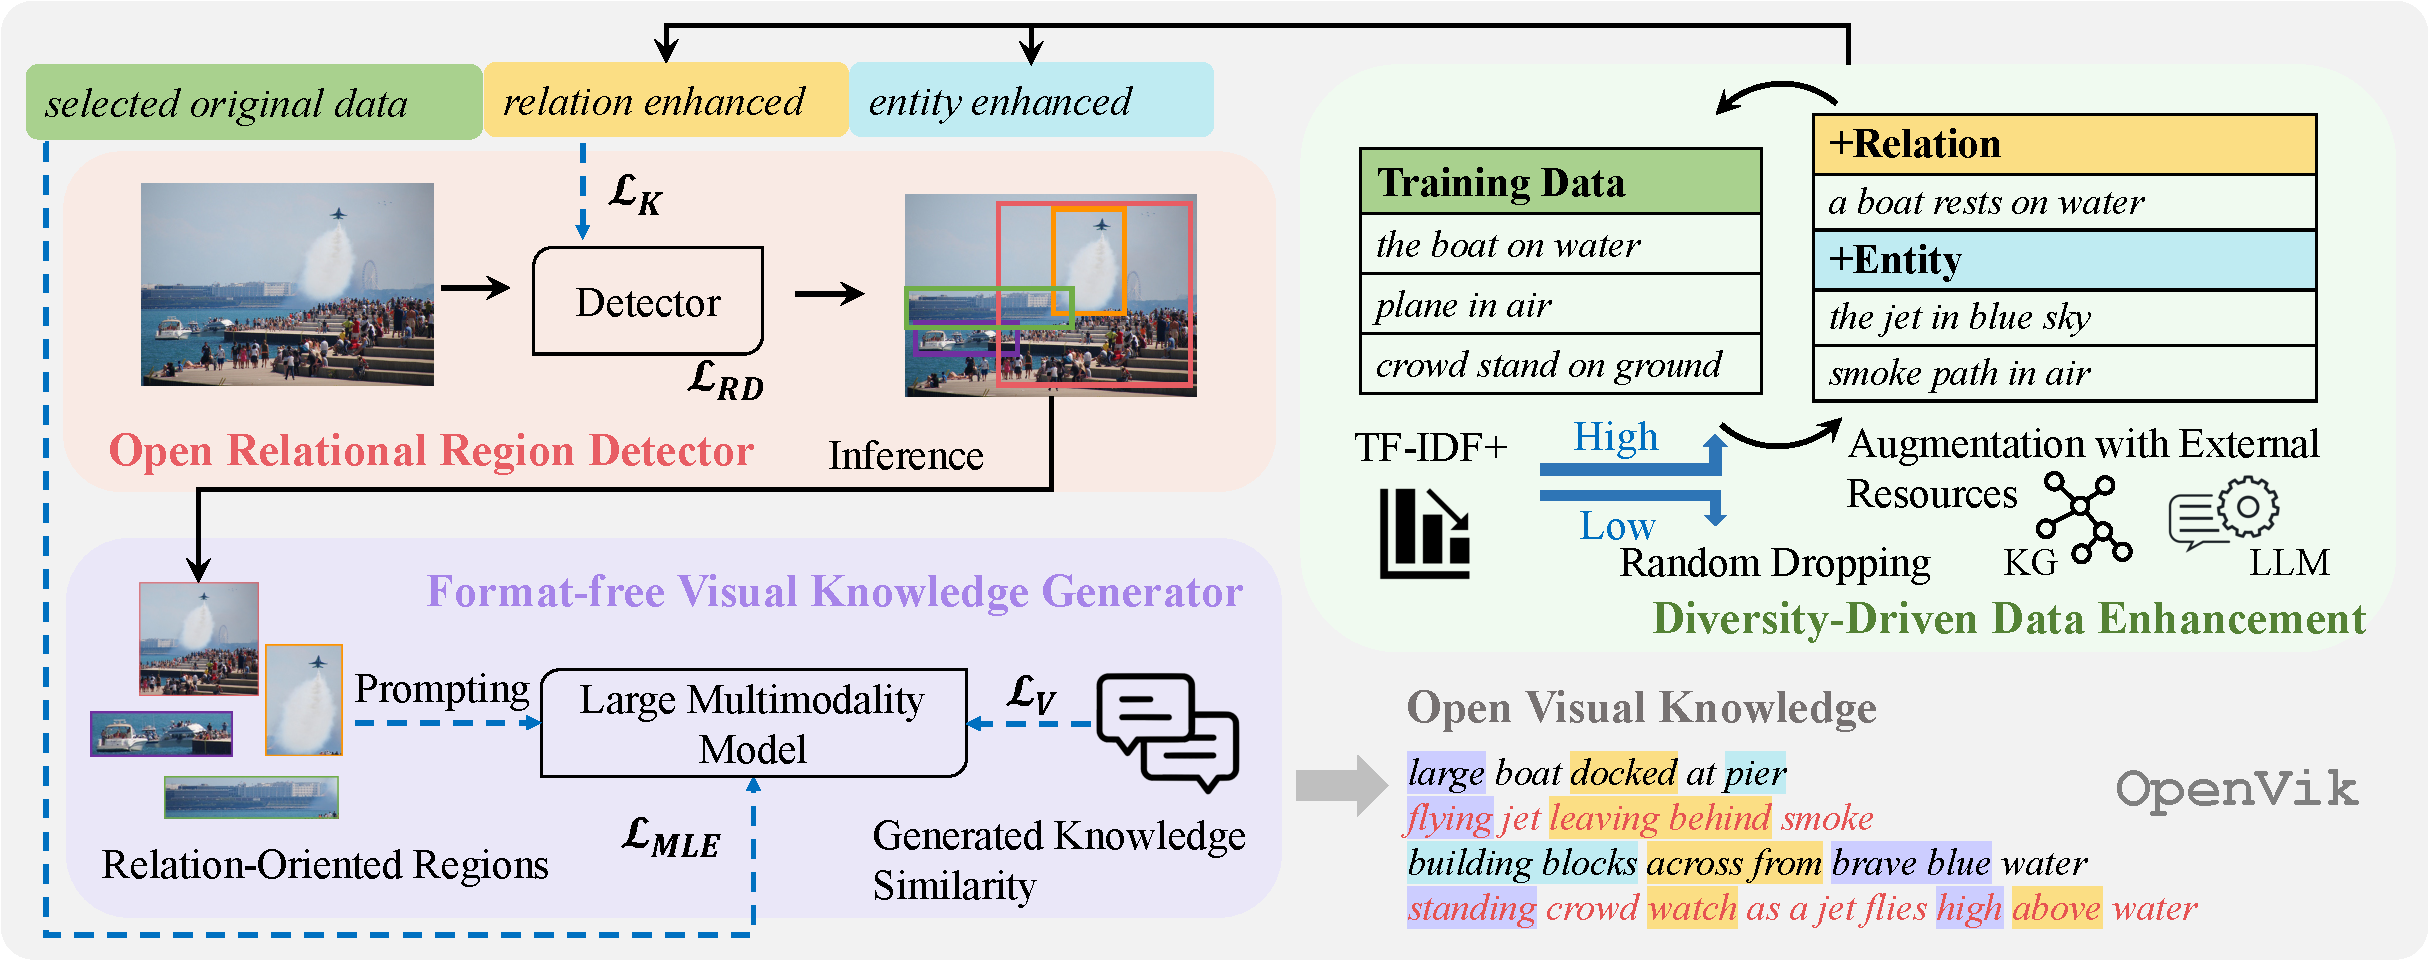
\includegraphics[width=.95\columnwidth]{submissions/CarlYang2024/figures/openvik.pdf}
    \end{center}
    % \vspace{-3mm}
    \caption{{The overall framework of OpenVik consists of two main components: (1) an open relational region detector, highlighted in the orange and purple panels, which includes a region regression loss ($\mathcal{L}_{\text{RD}}$) and a regional description loss ($\mathcal{L}_{\text{K}}$), and (2) a format-free visual knowledge generator, incorporating knowledge generation loss ($\mathcal{L}_{\text{MLE}}$) and diversity regularization ($\mathcal{L}_{\text{V}}$). These modules work collaboratively to extract open visual knowledge, incorporating novel entities and diverse relations in a format-free manner.}}
    \label{fig:openvik}
    % \vspace{-5mm}
\end{figure}



\subsection{Enriching KGs with multi-modality data}
Traditionally, specialized models and algorithms have been developed to process and analyze various modalities of data such as tables, texts, images, and time series. These methods can hardly perform integrative analysis across data modalities and generalize across different data platforms. Recently, LLM-based multi-modality foundation models (MMFMs) have shown strong promise in analyzing multi-modality data through the unified interface of languages \cite{yang2023dawn, fei2022towards, li2024multimodal, li2024llava, zhang2023biomedgpt}.
Integrating multi-modal data into KGs creates a more comprehensive representation of entities and their relationships, enhancing performance in open-world applications like image classification and visual question answering \cite{chen2024knowledge}. Many studies focus on using MMFMs for specific tasks, such as entity extraction \cite{sun2024umie,li2023prompting,hu2023prompt}, relation extraction \cite{yu2023visually,li2024zero,li2024pixels}, or event extraction \cite{chen2024schema,rasheed2024glamm}. However, these works often isolate extraction tasks without unifying entities and relations into a structured KG.
{A pioneering approach in this direction is OpenVik \cite{cui2024open} (framework shown in Figure~\ref{fig:openvik}). It first trains an open relational region detector to locate image regions containing relational information. 
It then employs a visual knowledge generator to create format-free knowledge descriptions by prompting a large visual language model. Through the use of MMFM, OpenVik advances KG completion by integrating rich visual context, expanding knowledge coverage, and enhancing the accuracy of representation within the resulting KG.}
Application-wise, Yang et al.~\cite{yang2024hierarchical}  proposed an automated approach to constructing product KGs from raw images in e-commerce. This method first employs vision-language models (VLMs) to extract detailed image information and then uses an LLM to reason and infer additional KG properties not visually present, hierarchically expanding, and linking nodes to develop comprehensive, scalable KGs without human input.


% https://www.cs.emory.edu/~jyang71/files/openvik.pdf